\chapter{Trabajo a futuro}\label{ch:futuro}
\chapterquote{To my future descendants: I have lent to Miss Bloop's private museum, the Medallion and the Ancestral Tunic which rightfully belong to you.}{Twinsen}

En este capítulo se hace una breve mención del trabajo que resta por hacer para completar la implementación del sistema conformador de haz, así como también posibles alternativas de implementación que no fueron estudiadas a lo largo de este proyecto y que pueden mejorar el producto final.

\section{Interfaz e integración con el sistema de adquisición}\label{subc:futuro_interfaz}
Como se mencionó en el Capítulo \ref{ch:sistema}, el fin de este sistema es ser implementado en una placa de desarrollo CIAA-ACC, sobre la cual va a estar instalado, también, el sistema de adquisición de muestras del ARU. Estos dos sistemas deben estar comunicados, de manera tal que el sistema de adquisición pueda enviar las muestras al sistema conformador de haz. Debido a que el conformador de haz tendrá parte de su implementación en el PS y parte de su implementación en la PL, es necesario definir las interfaces y el protocolo que utilizarán para la comunicación. En el chip Xilinx Zynq-7030, el PS puede comunicarse con la PL a través de un bus AXI-Lite, en el cual el PS toma el rol de maestro y la PL de esclavo. Por esto, es intuitivo pensar que dentro de la FPGA el sistema adquisidor y los bloques muestreador aleatorio y conformador de haz pueden tomar el rol de esclavos AXI y ser comandados por software a través del PS para redirigir las muestras al bloque estimador de DOA. Por otro lado, se puede evaluar el uso de una interfaz directa entre el sistema adquisidor y los bloques conformador de haz y muestreador aleatorio, ya que estos bloques deberán poder tener acceso simultáneamente a los registros del sistema adquisidor donde se almacenan las muestras de los elementos. Asegurarse una conexión punto a punto entre estos bloques es un criterio de diseño primordial para asegurar el mayor rendimiento del sistema. Finalmente, la interfaz entre el maestro AXI y el bloque estimador de DOA, dentro del PS, puede utilizar una interfaz UDP, debido a su simplicidad de implementación y a que en esta interfaz no se requiere verificar la integridad de los datos transmitidos. Además, si se decide utilizar GNU Radio para la ejecución de este bloque, este cuenta con una interfaz UDP que puede ser instanciada fácilmente con un bloque. En este caso deberá definirse, además, un protocolo de empaquetamiento de los datos transmitidos. En la Figura \ref{fig:futuro_interfaz} se muestra un esquema de esta propuesta.

\begin{figure}[ht!]
    \centering
    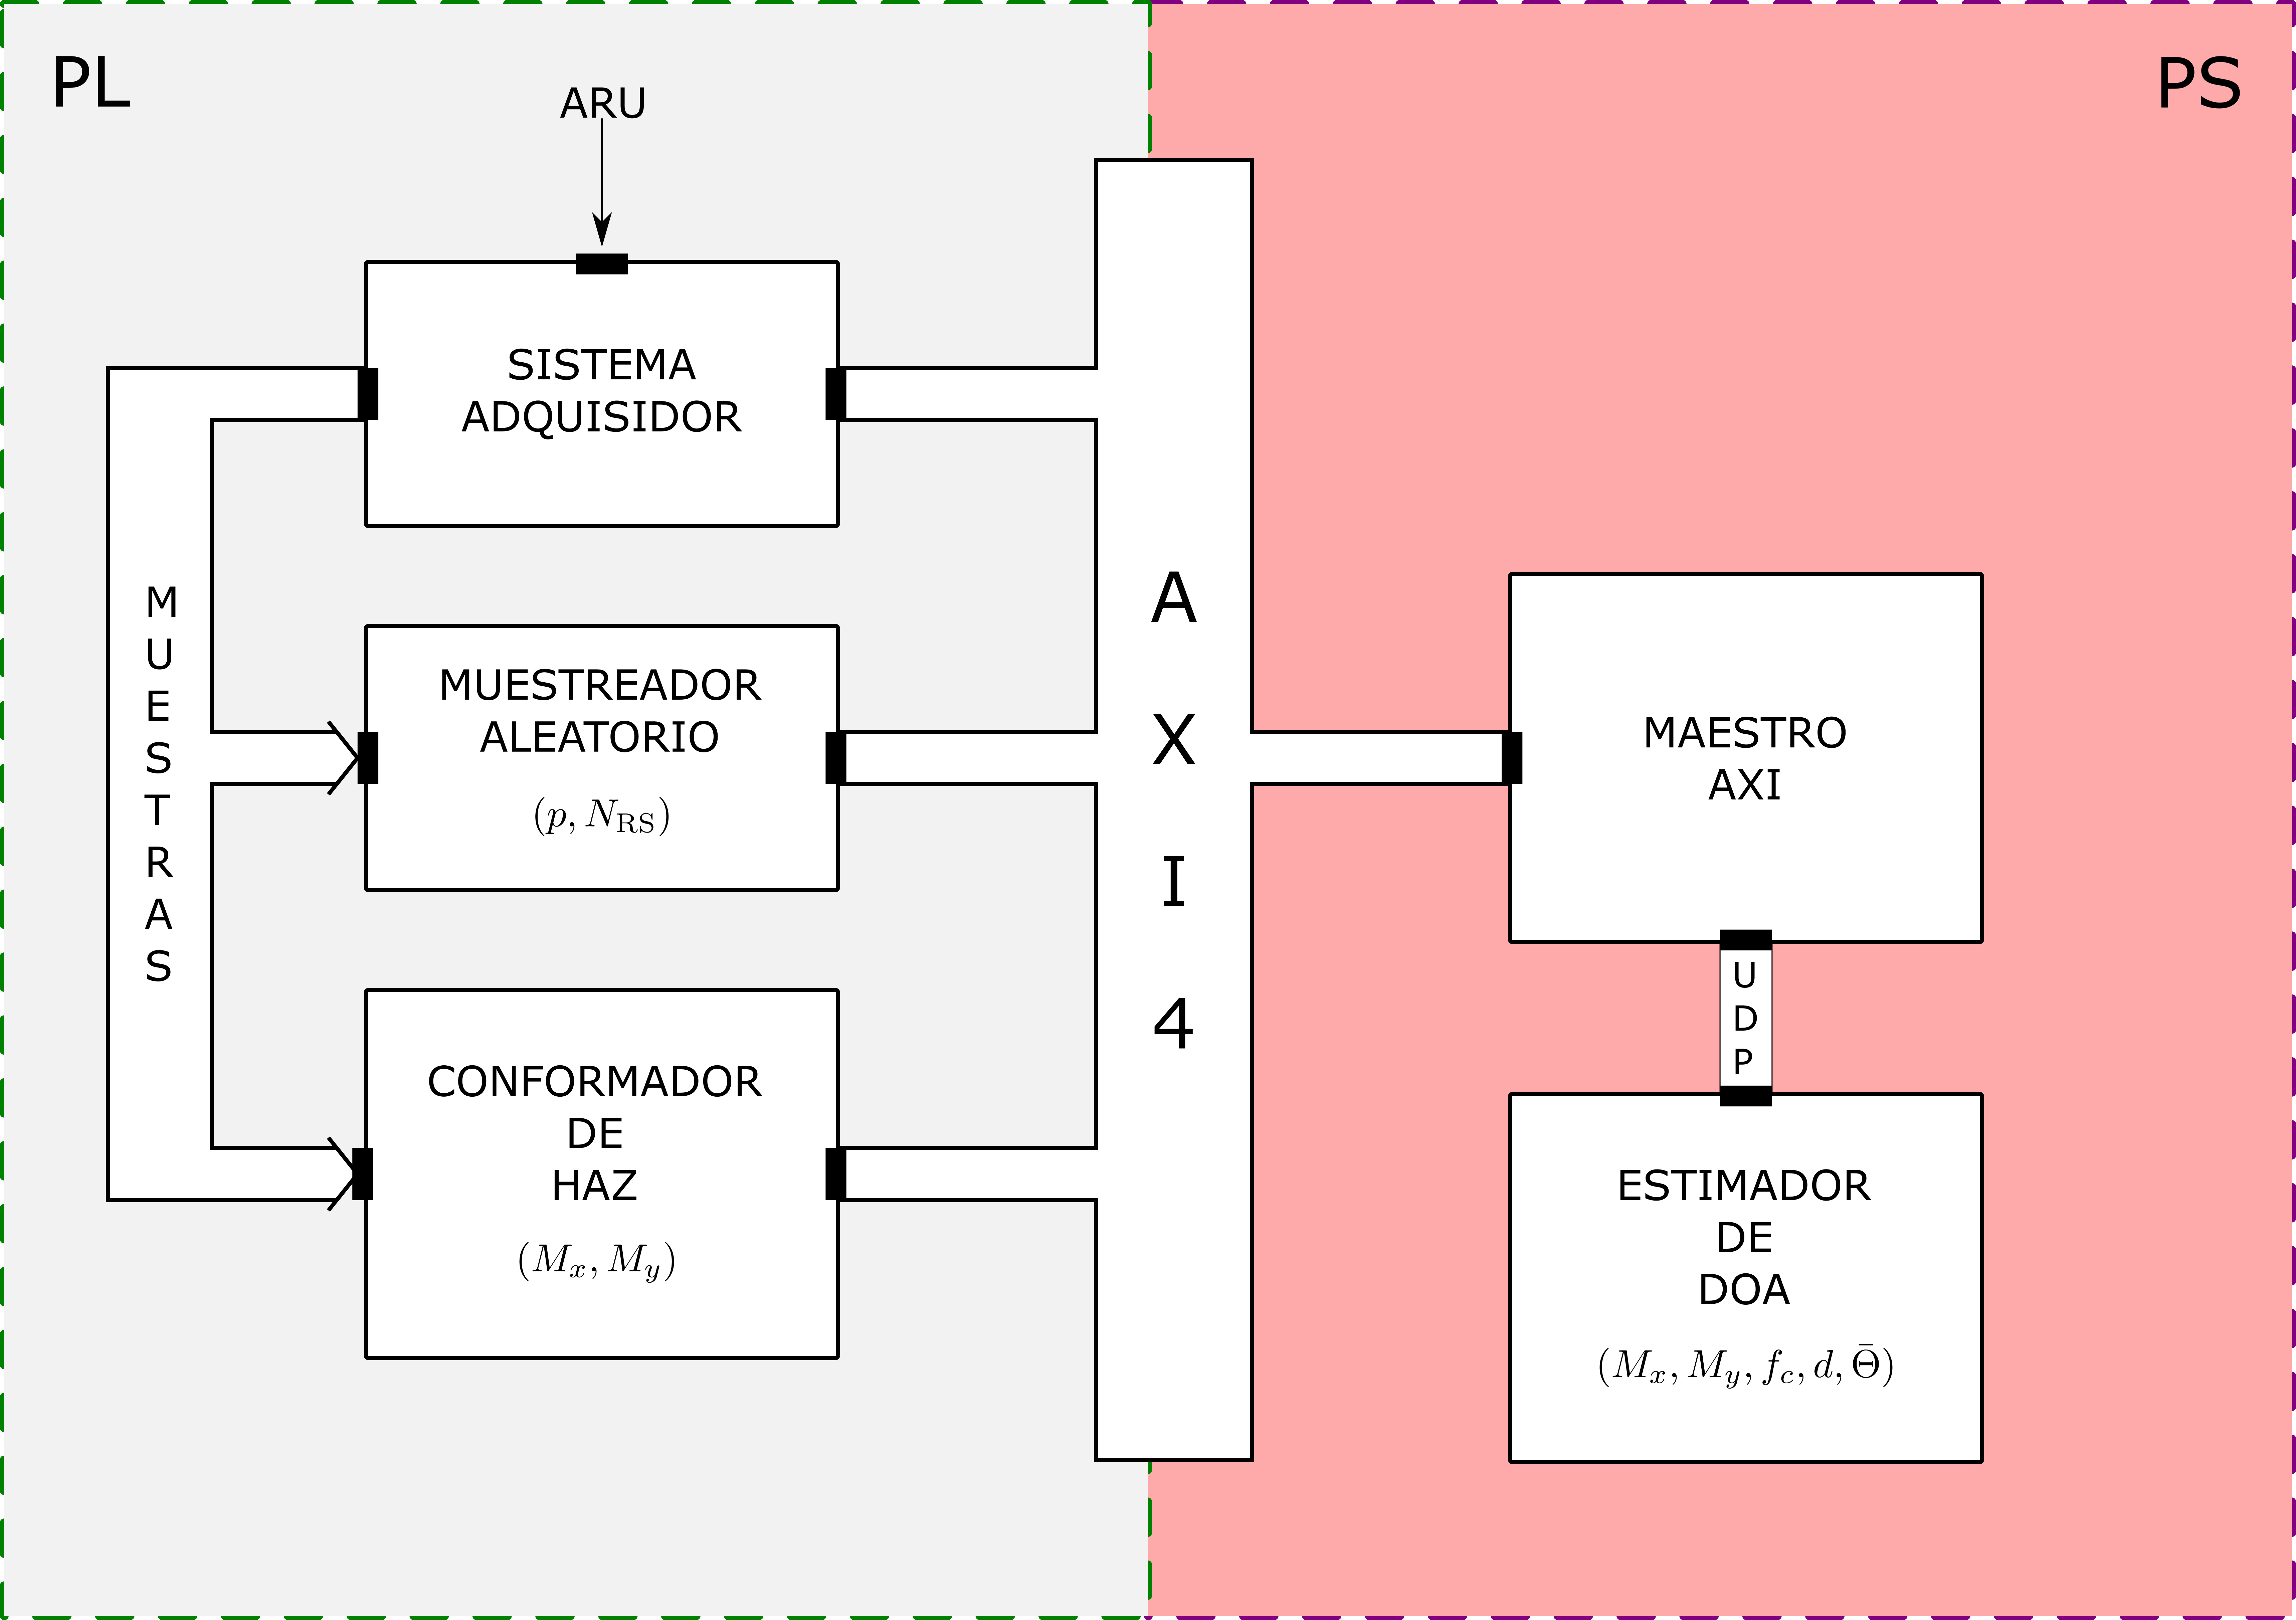
\includegraphics[width=0.9\linewidth]{images/08-Futuro/futuro_interfaz.png}
    \caption{Propuesta de interfaz para la integración del sistema conformador de haz con el sistema de adquisición.}
    \label{fig:futuro_interfaz}
\end{figure}

\section{Carga del patrón de radiación del arreglo}\label{subc:futuro_patron}
Una vez construido el arreglo de antenas con el cual se equipará el sistema, y habiendo realizado una medición de su patrón de radiación, debe cargarse esta información dentro del bloque conformador de haz para poder realizar la normalización de las muestras recibidas, como se mostró en la Sección \ref{subc:sistema_beamformer}.

\section{Interferencias destructivas}
Como se nombró en el Capítulo \ref{ch:beamforming}, la técnica de conformación de haz no solo permite realizar la recepción o transmisión direccional de señales sino que también permite generar mínimos en el patrón de radiación de manera tal de poder suprimir interferencias direccionales. La manera de generar estos mínimos es aplicando distintos pesos a las muestras provenientes de los elementos del arreglo. Una vez conocida la dirección de la interferencia, los pesos a aplicar pueden obtenerse mediante la resolución de un sistema de ecuaciones.

\section{Smart Beamforming}\label{subc_smartbeamforming}
Si bien el algoritmo que se desarrolló en este proyecto puede considerarse de alguna manera ``inteligente'' debido a que es capaz de deducir por su cuenta la dirección de arribo de señales, el término \emph{Smart Beamforming} hace referencia a técnicas de conformación de haz que utilizan algoritmos de inteligencia artificial para la estimación de DOA y la conformación de las señales arribantes.
Actualmente ya existen estudios que demuestran la factibilidad técnica y la mejora en rendimiento al emplear algoritmos de estimación de DOA basados en inteligencia artificial y, particularmente, en redes neuronales \cite{bib:smart_beamforming}, lo cual motiva a tener en cuenta este tipo de análisis para futuras implementaciones.